\documentclass{article}
\usepackage{graphicx}
\usepackage[utf8]{inputenc}
\usepackage[T1]{fontenc}
\usepackage{lmodern}
\usepackage{float}
\usepackage{caption}
\usepackage{subcaption}
\usepackage[paperwidth=4.1in, paperheight=5.8in, margin=0.25in]{geometry}
\renewcommand*\familydefault{\sfdefault}
\pagenumbering{gobble}

\usepackage{pgfmorepages}

\pgfpagesdeclarelayout{8 on 2, book format}
{%
  \edef\pgfpageoptionheight{\the\paperheight}
  \edef\pgfpageoptionwidth{\the\paperwidth}
  \def\pgfpageoptionborder{0pt}
  \def\pgfpageoptionfirstshipout{1}
}%
{%
  \pgfpagesphysicalpageoptions
  {%
    logical pages=8,%
    physical pages=2,%
    physical height=\pgfpageoptionheight,%
    physical width=\pgfpageoptionwidth,%
    current logical shipout=\pgfpageoptionfirstshipout%
  }
  \pgfpagesphysicalpage{1}{}
    \pgfpageslogicalpageoptions{4}
    {%
      border shrink=\pgfpageoptionborder,%
      resized width=.5\pgfphysicalwidth,%
      resized height=.5\pgfphysicalheight,%
      center=\pgfpoint{.25\pgfphysicalwidth}{.75\pgfphysicalheight}%
    }%
    \pgfpageslogicalpageoptions{2}
    {%
      border shrink=\pgfpageoptionborder,%
      resized width=.5\pgfphysicalwidth,%
      resized height=.5\pgfphysicalheight,%
      center=\pgfpoint{.75\pgfphysicalwidth}{.75\pgfphysicalheight}%
    }%
    \pgfpageslogicalpageoptions{8}
    {%
      border shrink=\pgfpageoptionborder,%
      resized width=.5\pgfphysicalwidth,%
      resized height=.5\pgfphysicalheight,%
      center=\pgfpoint{.25\pgfphysicalwidth}{.25\pgfphysicalheight},%
    }%
    \pgfpageslogicalpageoptions{6}
    {%
      border shrink=\pgfpageoptionborder,%
      resized width=.5\pgfphysicalwidth,%
      resized height=.5\pgfphysicalheight,%
      center=\pgfpoint{.75\pgfphysicalwidth}{.25\pgfphysicalheight},%
    }%
  \pgfpagesphysicalpage{2}{}
    \pgfpageslogicalpageoptions{1}
    {%
      border shrink=\pgfpageoptionborder,%
      resized width=.5\pgfphysicalwidth,%
      resized height=.5\pgfphysicalheight,%
      center=\pgfpoint{.25\pgfphysicalwidth}{.75\pgfphysicalheight}%
    }%
    \pgfpageslogicalpageoptions{3}
    {%
      border shrink=\pgfpageoptionborder,%
      resized width=.5\pgfphysicalwidth,%
      resized height=.5\pgfphysicalheight,%
      center=\pgfpoint{.75\pgfphysicalwidth}{.75\pgfphysicalheight}%
    }%
    \pgfpageslogicalpageoptions{5}
    {%
      border shrink=\pgfpageoptionborder,%
      resized width=.5\pgfphysicalwidth,%
      resized height=.5\pgfphysicalheight,%
      center=\pgfpoint{.25\pgfphysicalwidth}{.25\pgfphysicalheight},%
    }%
    \pgfpageslogicalpageoptions{7}
    {%
      border shrink=\pgfpageoptionborder,%
      resized width=.5\pgfphysicalwidth,%
      resized height=.5\pgfphysicalheight,%
      center=\pgfpoint{.75\pgfphysicalwidth}{.25\pgfphysicalheight},%
    }%
}


\pgfpagesuselayout{8 on 2, book format}[a4paper]
\begin{document}
    
        \par\noindent\rule{\textwidth}{0.4pt}
    \begin{figure}[H]
        \centering
        \begin{minipage}{0.25\textwidth}
            \centering
            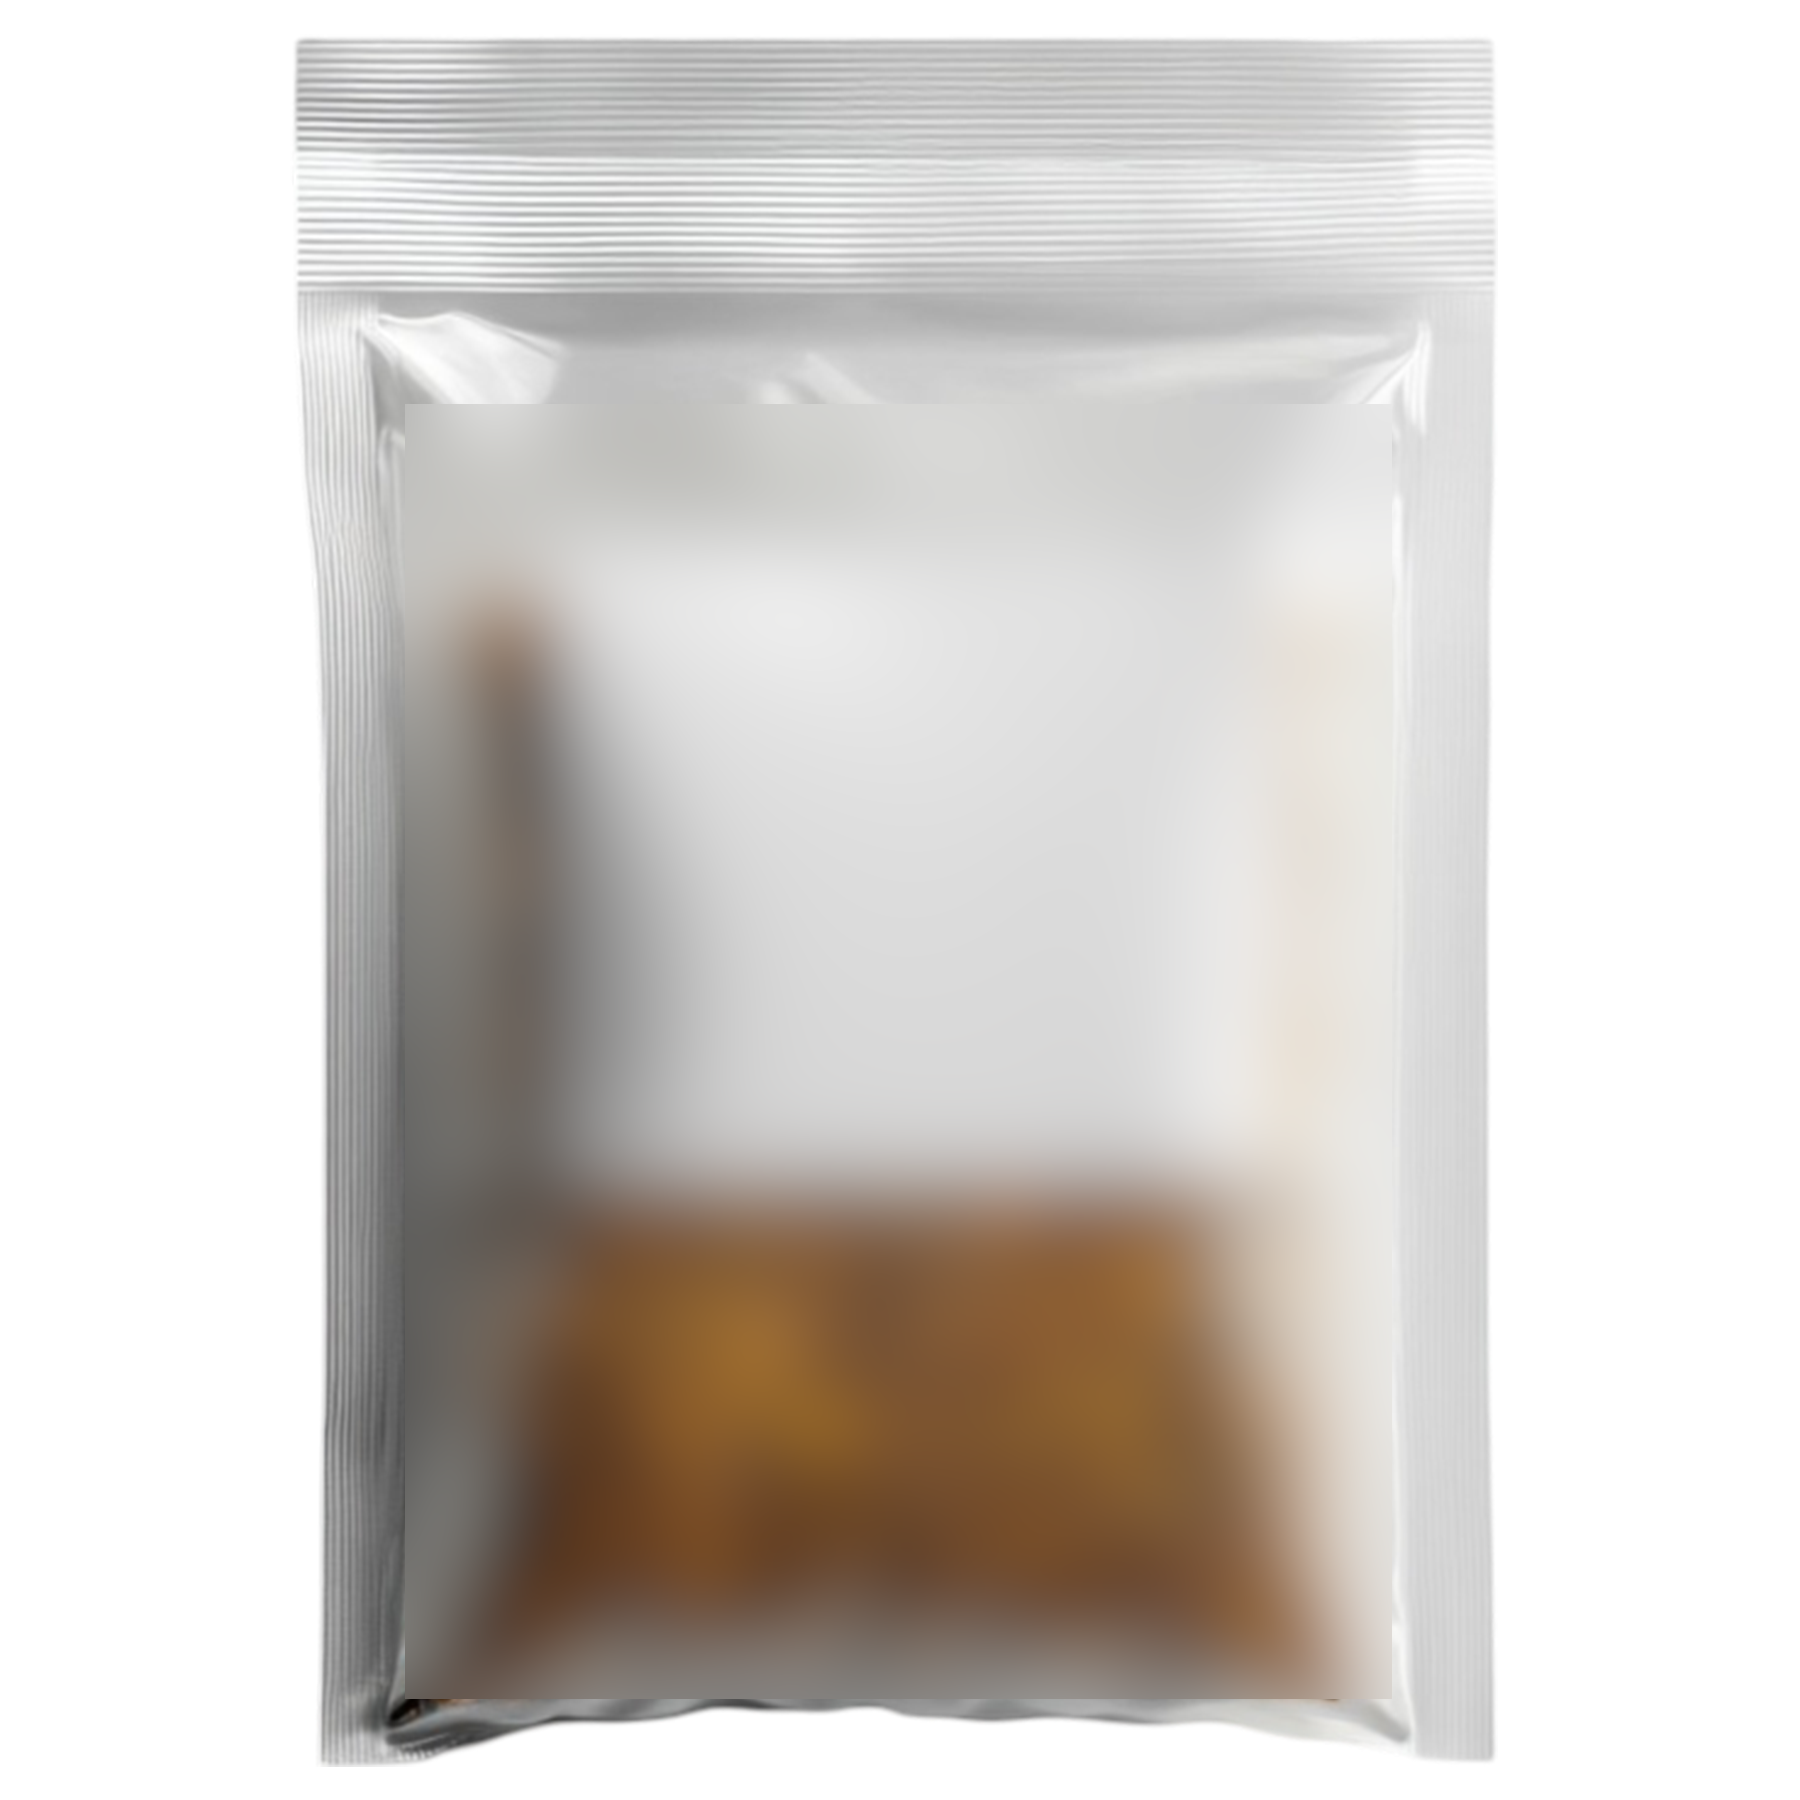
\includegraphics[width=\textwidth]{../SurvivalItemImages/concentrate}
        \end{minipage}\hfill
        \begin{minipage}{0.7\textwidth}
            \centering
            \Large Food concentrate
        \end{minipage}
    \end{figure}
    \vspace{-0.8em}
    \noindent\rule{\textwidth}{0.4pt}
            
    \begin{figure}[H]
        \centering
        \begin{minipage}{0.25\textwidth}
            \centering
            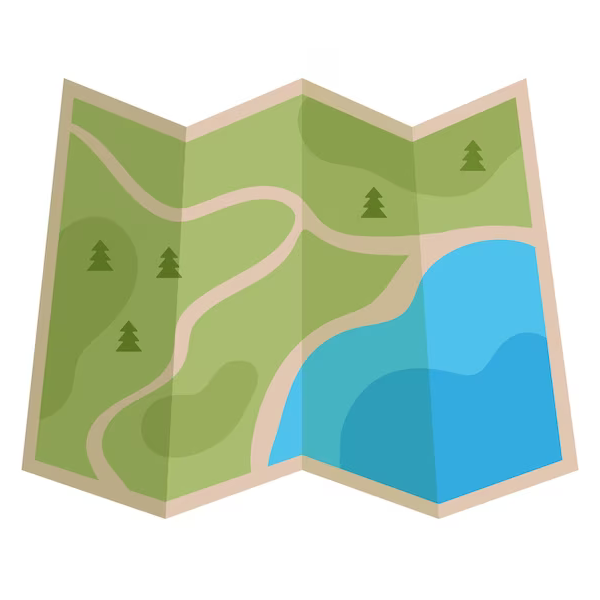
\includegraphics[width=\textwidth]{../SurvivalItemImages/map}
        \end{minipage}\hfill
        \begin{minipage}{0.7\textwidth}
            \centering
            \Large Stellar map
        \end{minipage}
    \end{figure}
    \vspace{-0.8em}
    \noindent\rule{\textwidth}{0.4pt}
            
    \begin{figure}[H]
        \centering
        \begin{minipage}{0.25\textwidth}
            \centering
            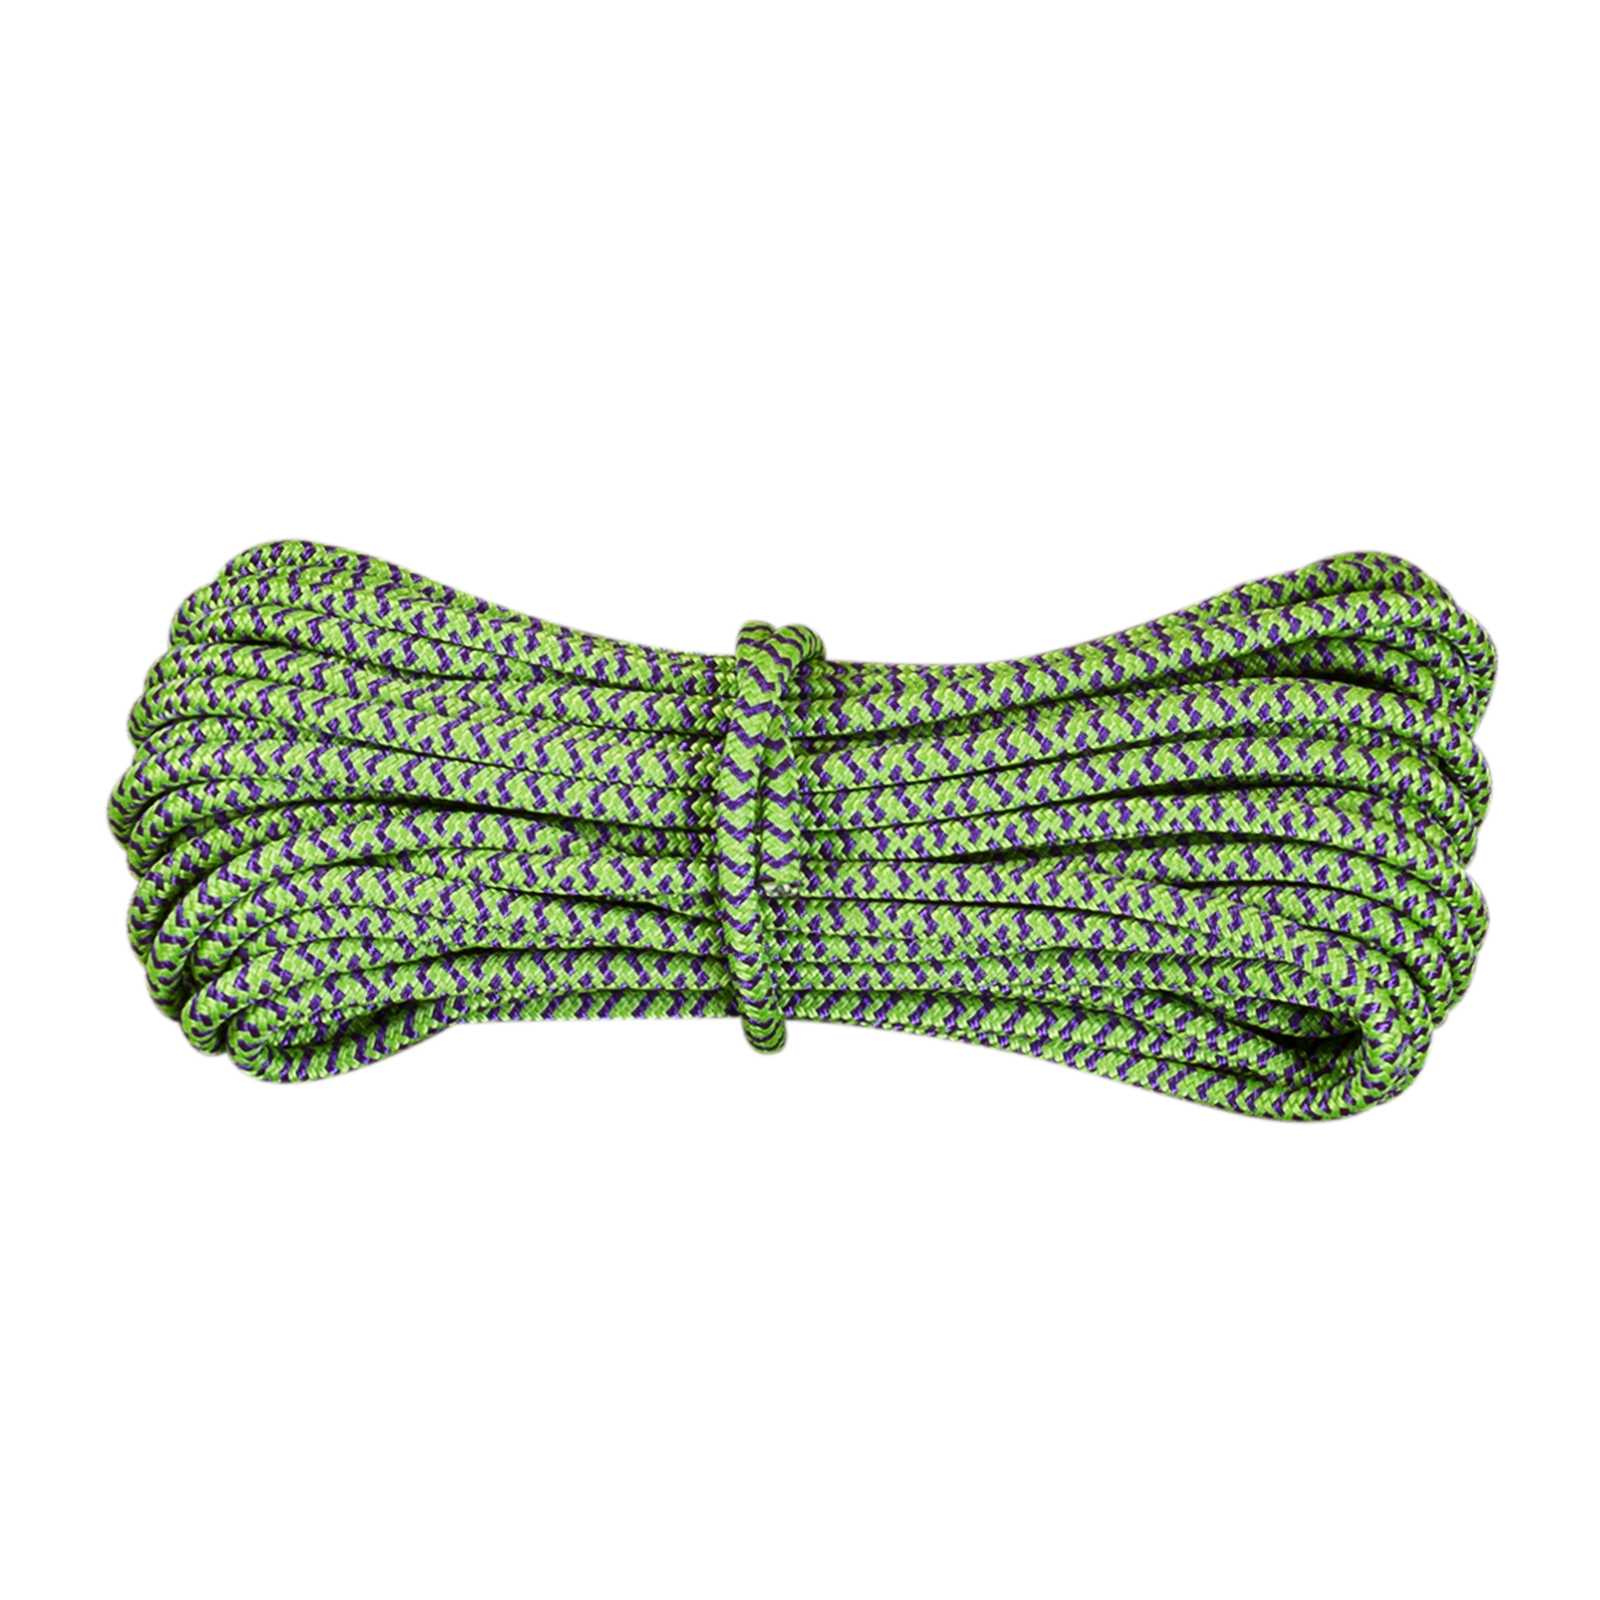
\includegraphics[width=\textwidth]{../SurvivalItemImages/rope}
        \end{minipage}\hfill
        \begin{minipage}{0.7\textwidth}
            \centering
            \Large 15 metres of nylon rope
        \end{minipage}
    \end{figure}
    \vspace{-0.8em}
    \noindent\rule{\textwidth}{0.4pt}
            
    \begin{figure}[H]
        \centering
        \begin{minipage}{0.25\textwidth}
            \centering
            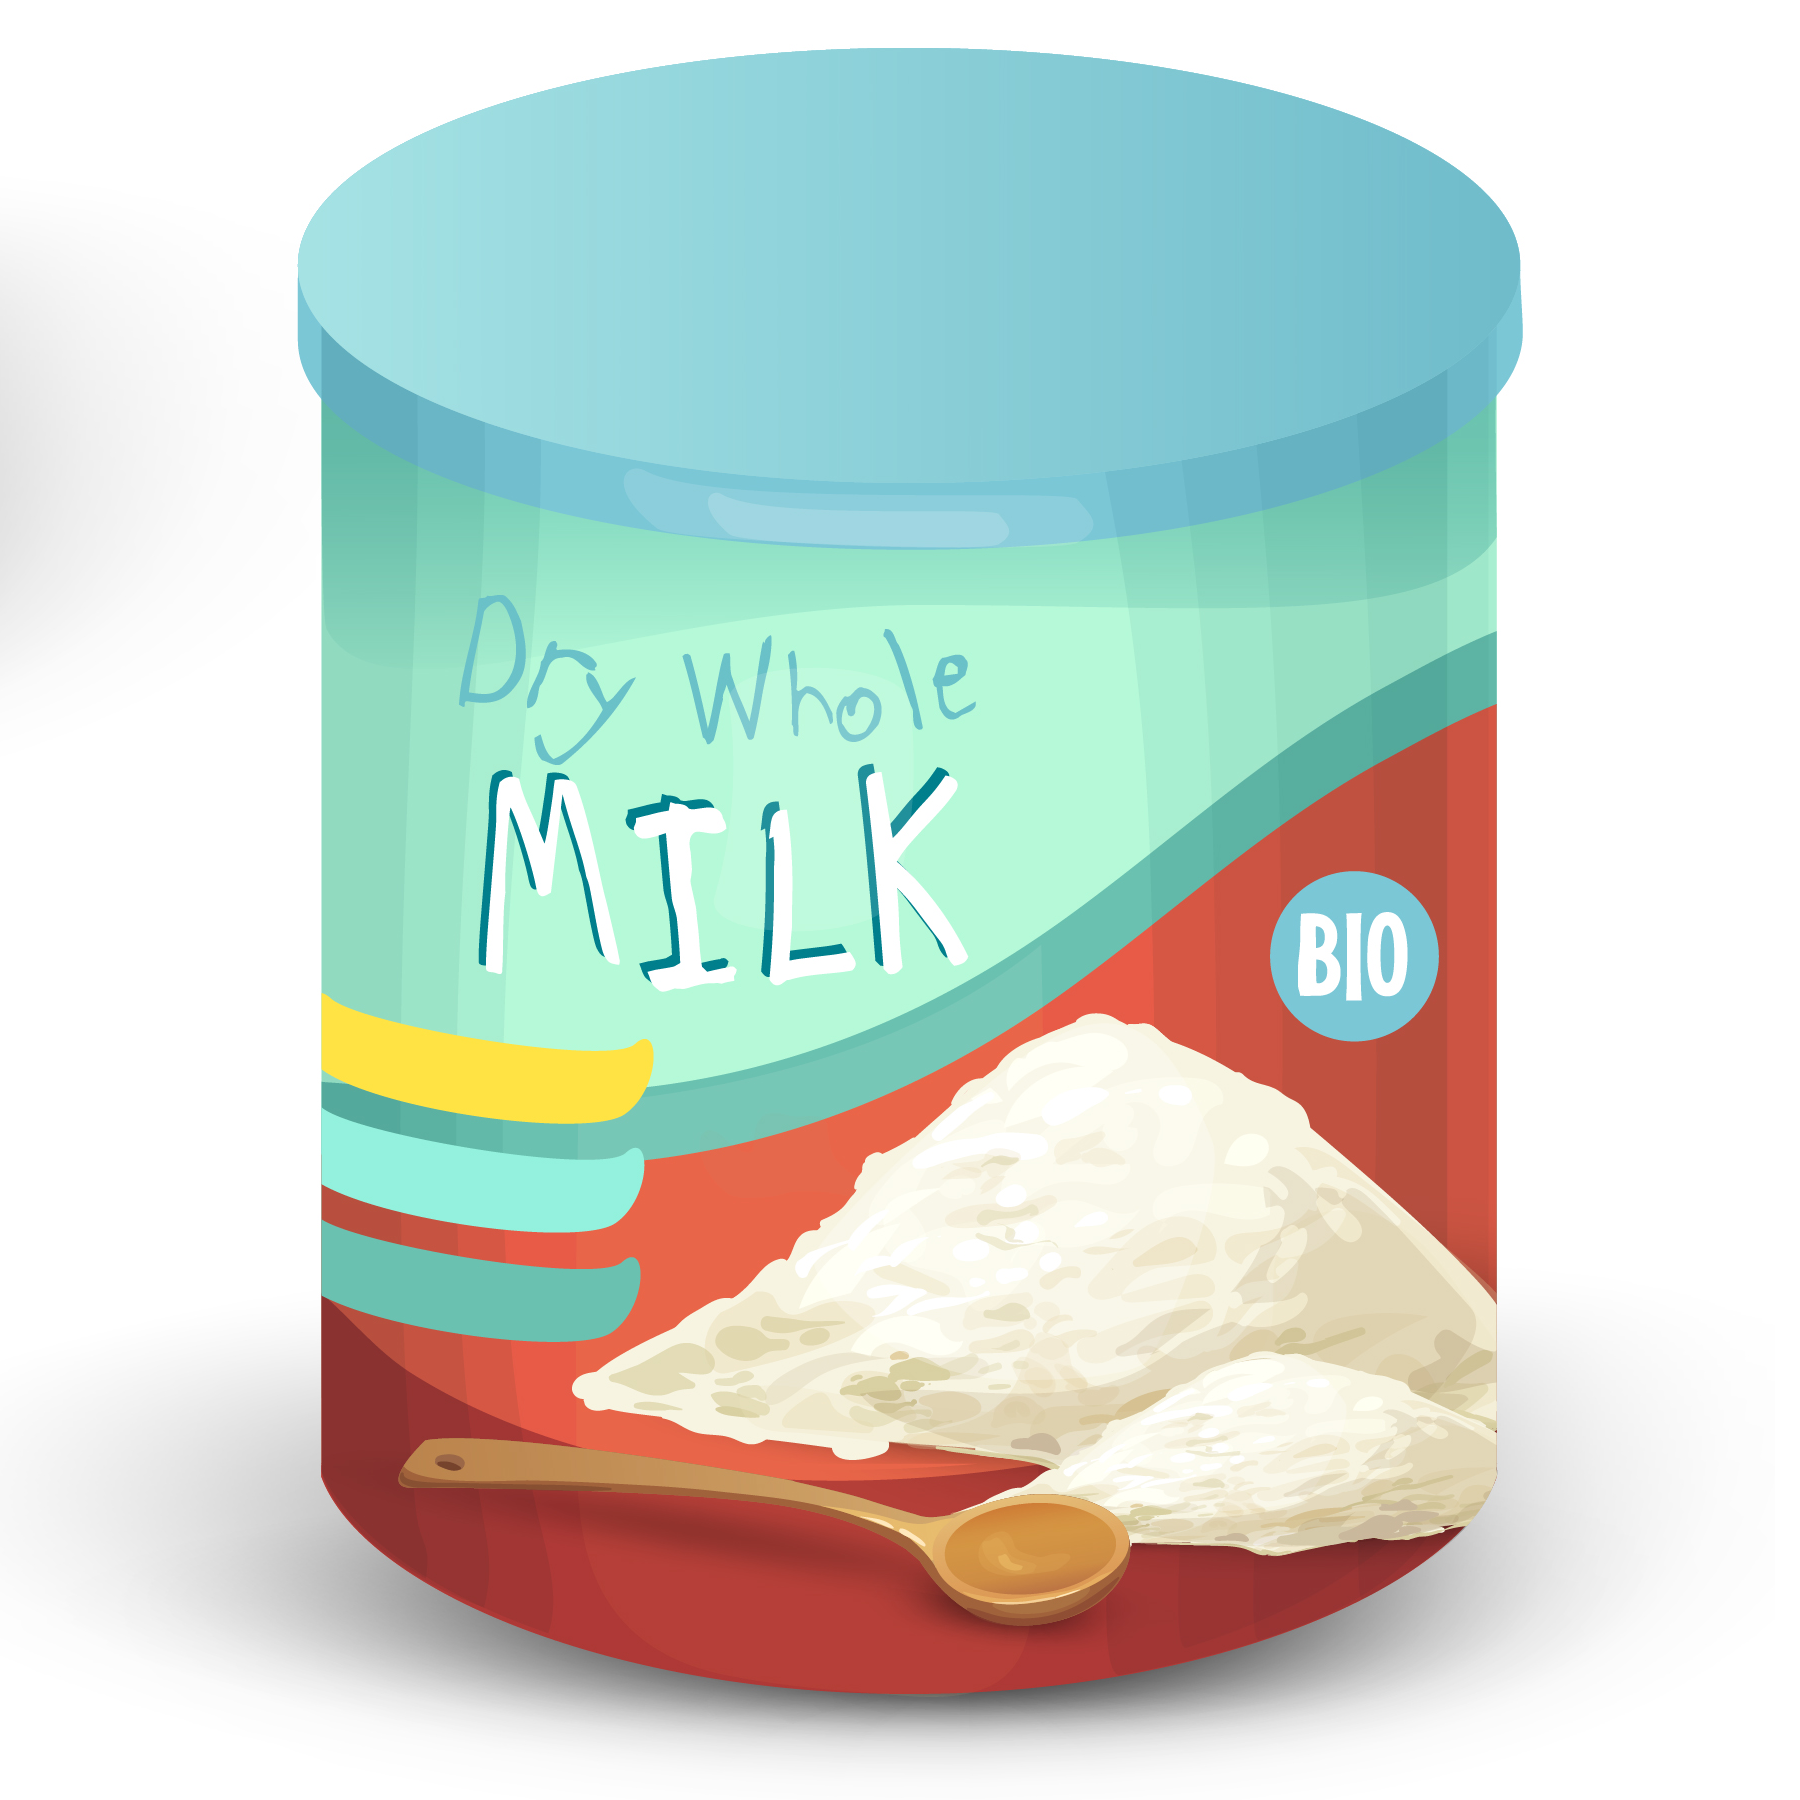
\includegraphics[width=\textwidth]{../SurvivalItemImages/milk}
        \end{minipage}\hfill
        \begin{minipage}{0.7\textwidth}
            \centering
            \Large One case of dehydrated milk
        \end{minipage}
    \end{figure}
    \vspace{-0.8em}
    \noindent\rule{\textwidth}{0.4pt}
            
    \clearpage
    \section*{Scenario: \textmd{Moon} \hfill Participant \textmd{0}}
    \Large You are a member of a space crew originally scheduled to rendezvous with a mother ship on the lighted surface of the moon. However, due to mechanical difficulties, your ship was forced to land at a spot some 200 miles from the rendezvous point. In addition to your space suit, your crew has managed to save items left intact and undamaged after landing. Your task is to take the items which allow you to reach the mother ship.
\clearpage
        \par\noindent\rule{\textwidth}{0.4pt}
    \begin{figure}[H]
        \centering
        \begin{minipage}{0.25\textwidth}
            \centering
            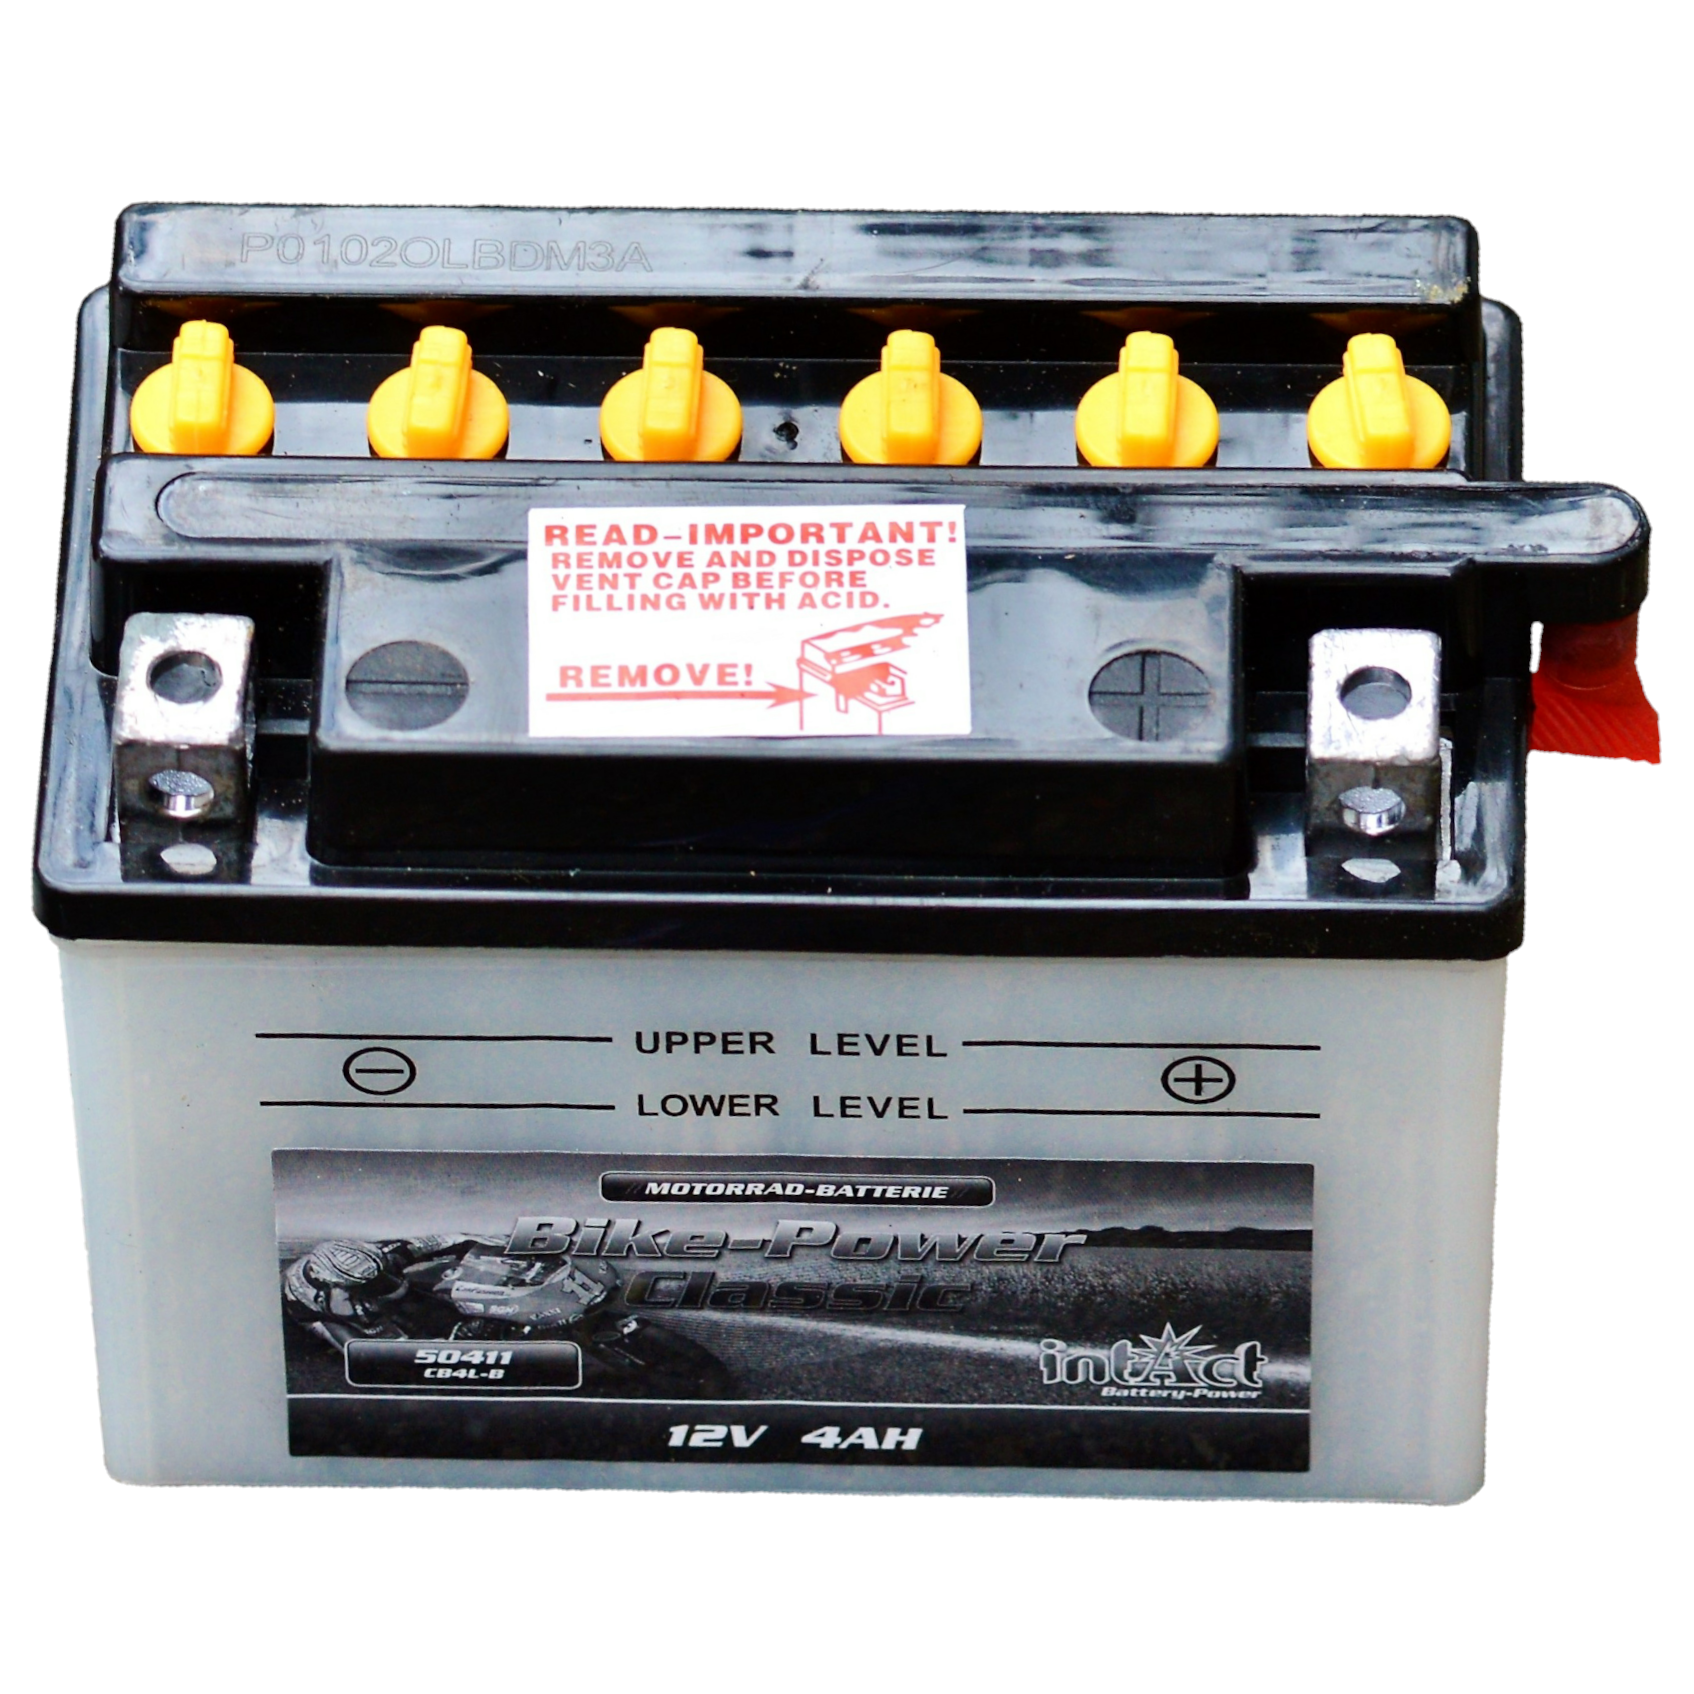
\includegraphics[width=\textwidth]{../SurvivalItemImages/battery}
        \end{minipage}\hfill
        \begin{minipage}{0.7\textwidth}
            \centering
            \Large  One battery set
        \end{minipage}
    \end{figure}
    \vspace{-0.8em}
    \noindent\rule{\textwidth}{0.4pt}
            
    \begin{figure}[H]
        \centering
        \begin{minipage}{0.25\textwidth}
            \centering
            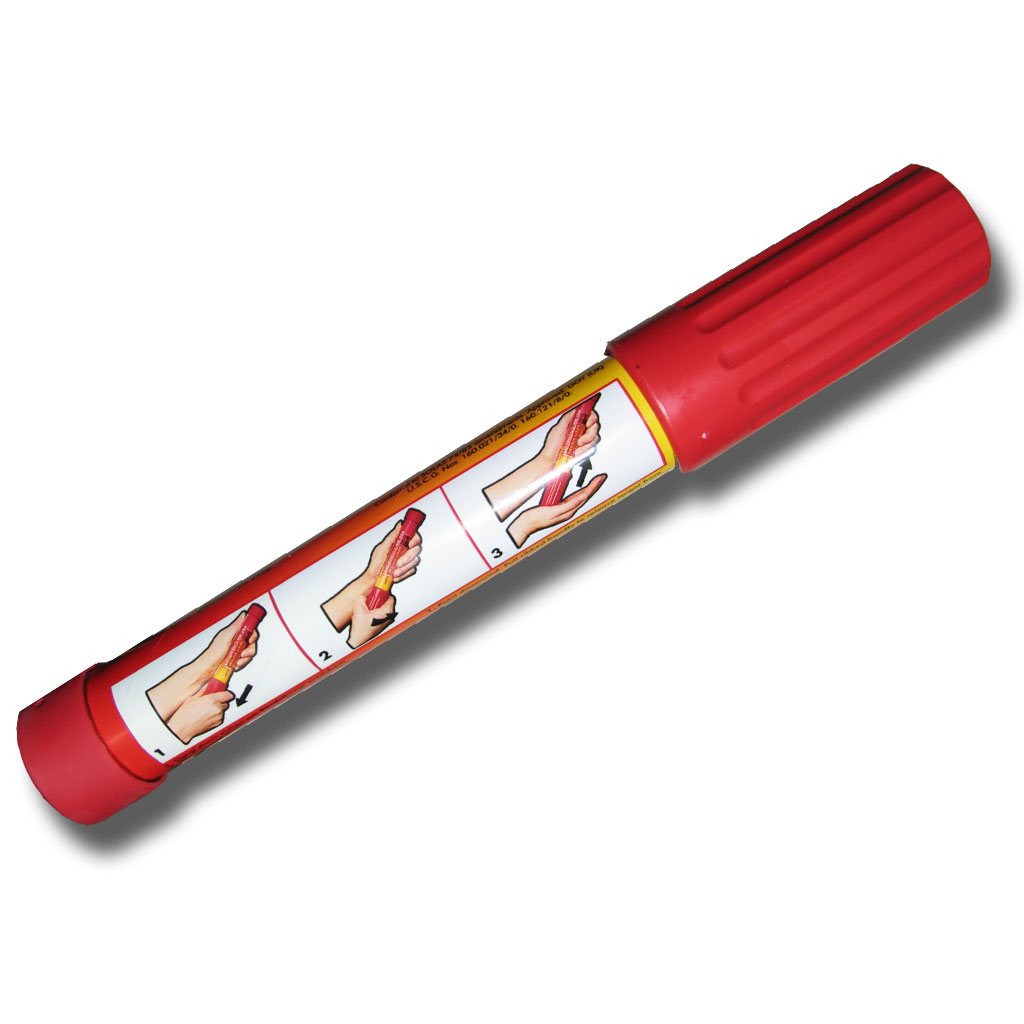
\includegraphics[width=\textwidth]{../SurvivalItemImages/flares}
        \end{minipage}\hfill
        \begin{minipage}{0.7\textwidth}
            \centering
            \Large Three signal flares
        \end{minipage}
    \end{figure}
    \vspace{-0.8em}
    \noindent\rule{\textwidth}{0.4pt}
            
    \begin{figure}[H]
        \centering
        \begin{minipage}{0.25\textwidth}
            \centering
            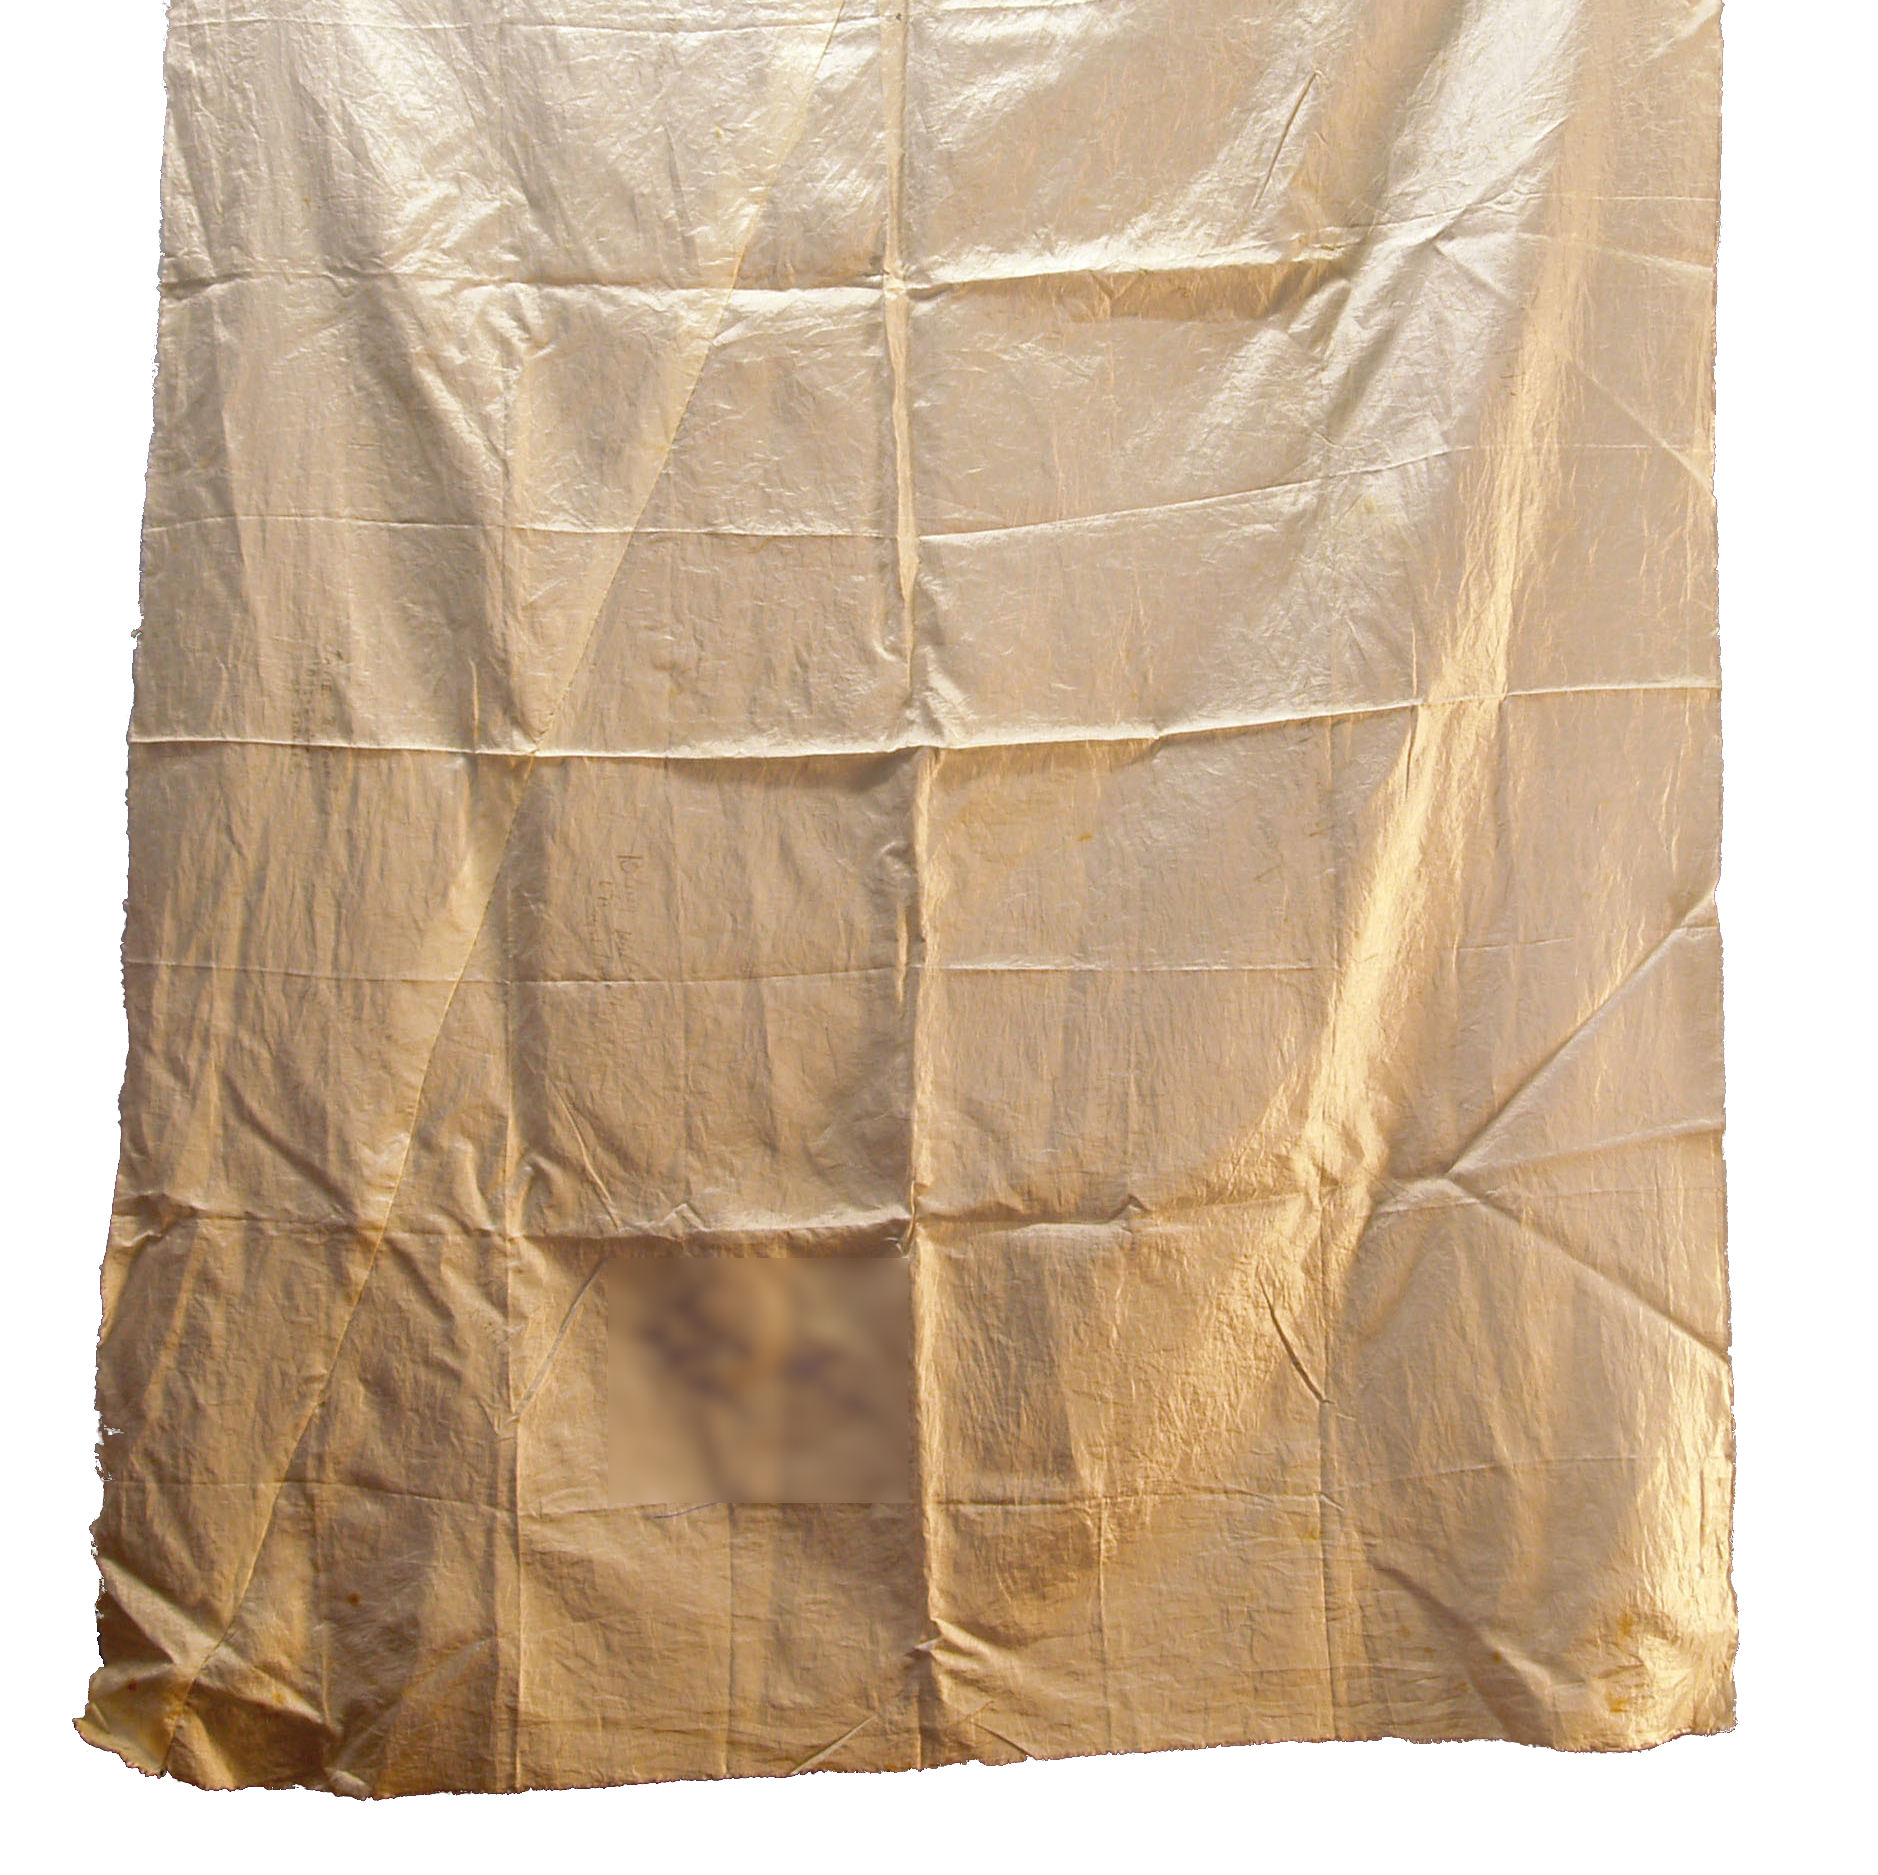
\includegraphics[width=\textwidth]{../SurvivalItemImages/silk}
        \end{minipage}\hfill
        \begin{minipage}{0.7\textwidth}
            \centering
            \Large Parachute silk
        \end{minipage}
    \end{figure}
    \vspace{-0.8em}
    \noindent\rule{\textwidth}{0.4pt}
            
    \begin{figure}[H]
        \centering
        \begin{minipage}{0.25\textwidth}
            \centering
            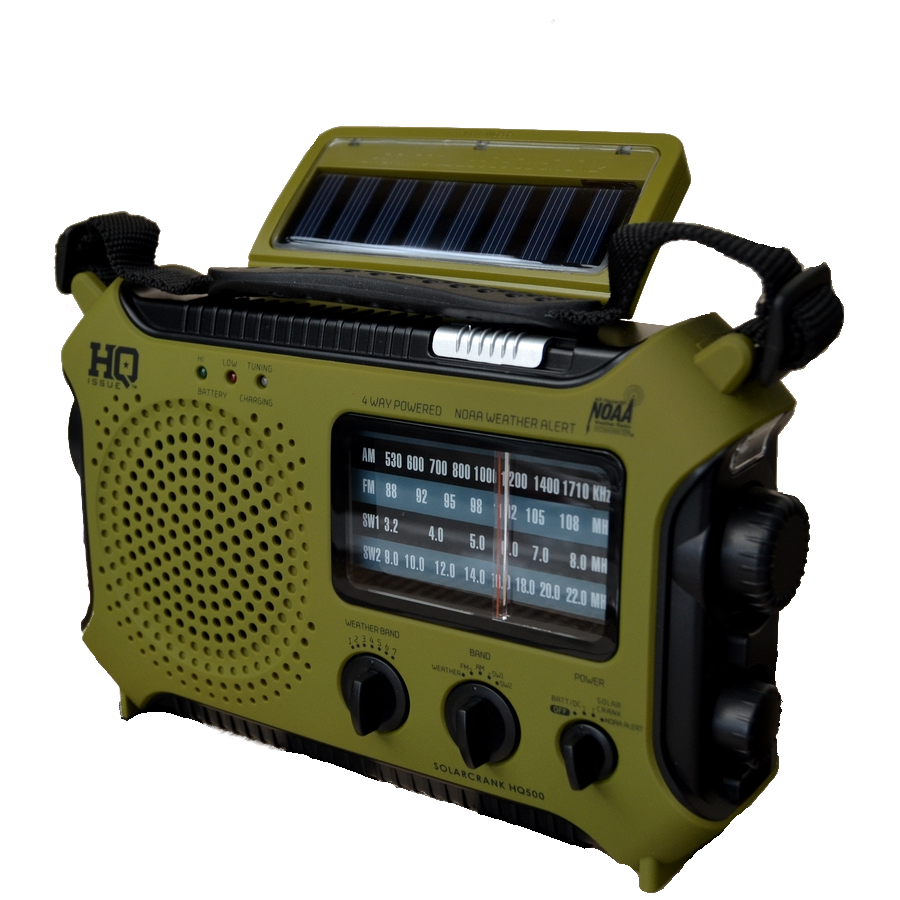
\includegraphics[width=\textwidth]{../SurvivalItemImages/transmitter}
        \end{minipage}\hfill
        \begin{minipage}{0.7\textwidth}
            \centering
            \Large Solar-powered FM receiver-transmitter
        \end{minipage}
    \end{figure}
    \vspace{-0.8em}
    \noindent\rule{\textwidth}{0.4pt}
            
    \clearpage
    \section*{Scenario: \textmd{Moon} \hfill Participant \textmd{1}}
    \Large You are a member of a space crew originally scheduled to rendezvous with a mother ship on the lighted surface of the moon. However, due to mechanical difficulties, your ship was forced to land at a spot some 200 miles from the rendezvous point. In addition to your space suit, your crew has managed to save items left intact and undamaged after landing. Your task is to take the items which allow you to reach the mother ship.
\clearpage
        \par\noindent\rule{\textwidth}{0.4pt}
    \begin{figure}[H]
        \centering
        \begin{minipage}{0.25\textwidth}
            \centering
            \includegraphics[width=\textwidth]{../SurvivalItemImages/firstaidkit}
        \end{minipage}\hfill
        \begin{minipage}{0.7\textwidth}
            \centering
            \Large First aid kit
        \end{minipage}
    \end{figure}
    \vspace{-0.8em}
    \noindent\rule{\textwidth}{0.4pt}
            
    \begin{figure}[H]
        \centering
        \begin{minipage}{0.25\textwidth}
            \centering
            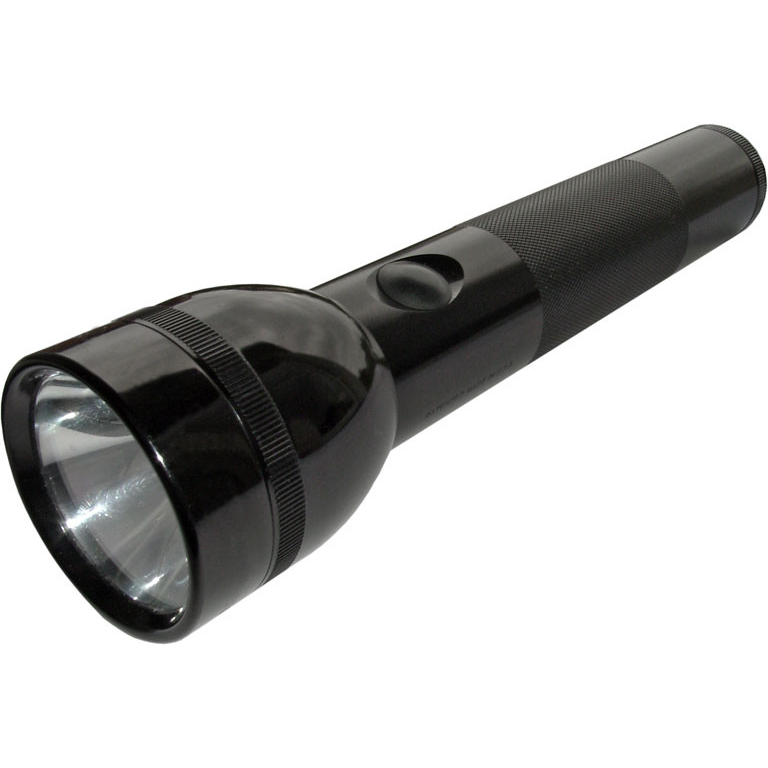
\includegraphics[width=\textwidth]{../SurvivalItemImages/torch}
        \end{minipage}\hfill
        \begin{minipage}{0.7\textwidth}
            \centering
            \Large A torch
        \end{minipage}
    \end{figure}
    \vspace{-0.8em}
    \noindent\rule{\textwidth}{0.4pt}
            
    \begin{figure}[H]
        \centering
        \begin{minipage}{0.25\textwidth}
            \centering
            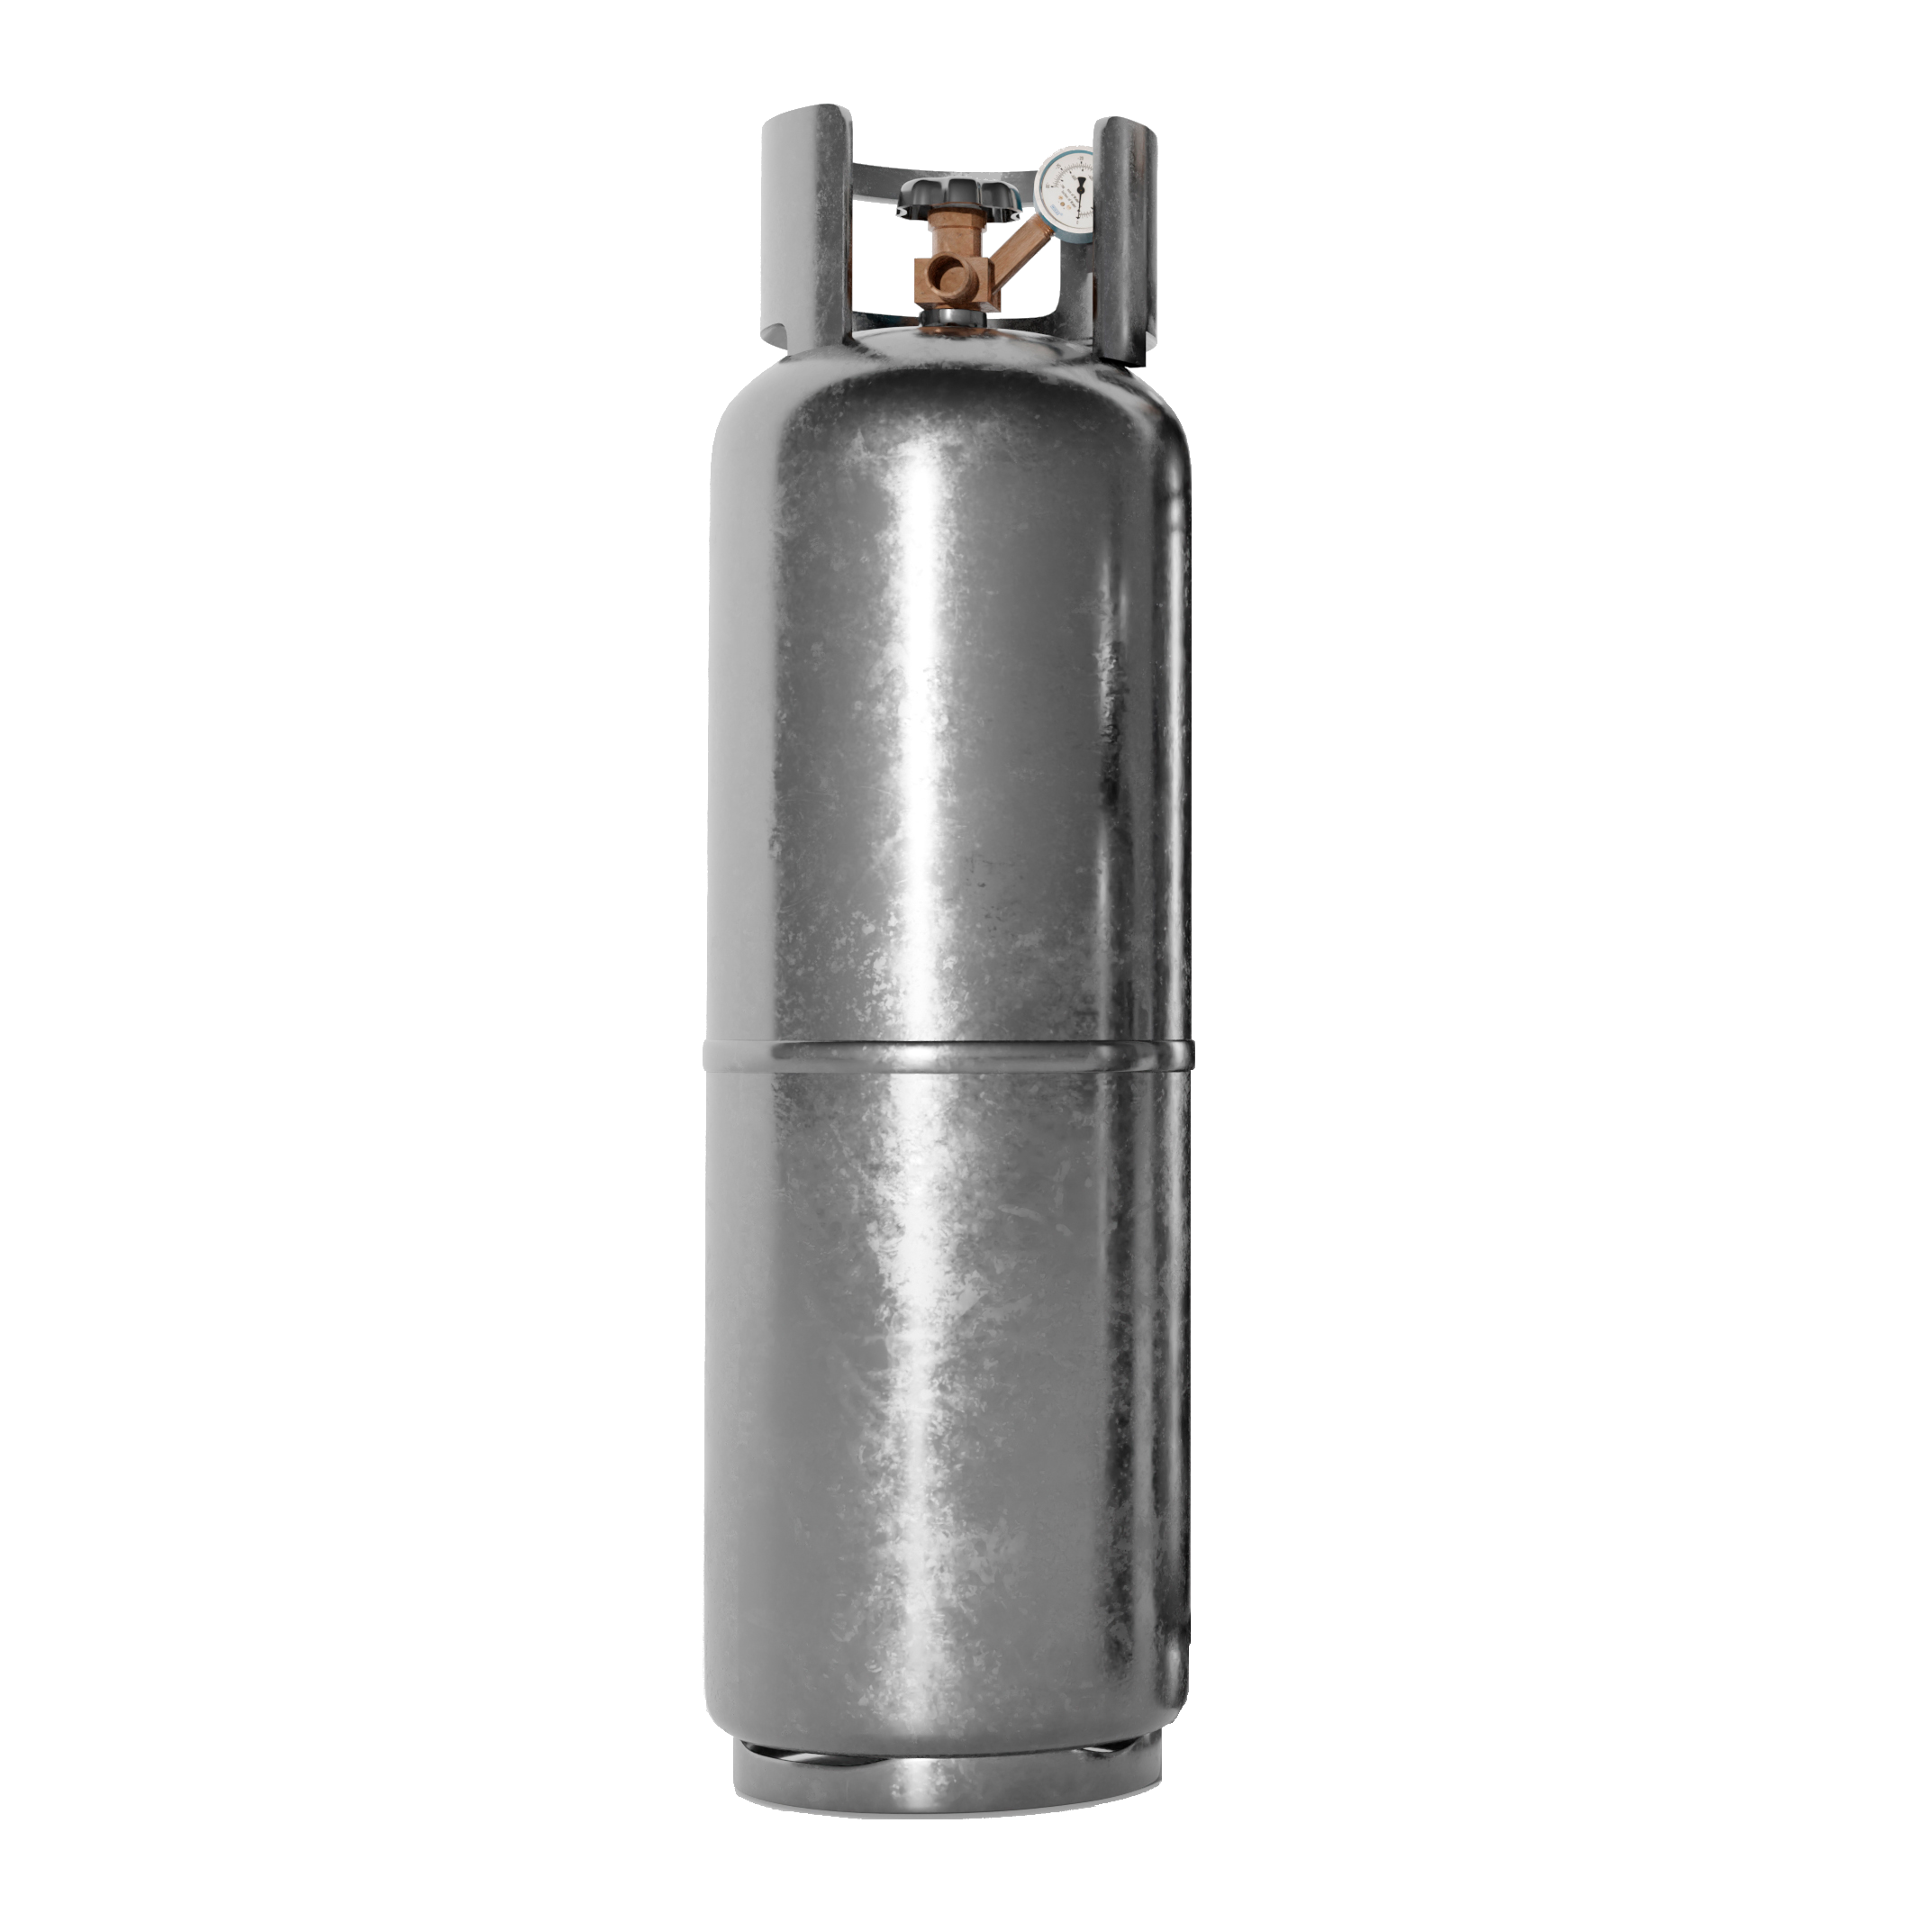
\includegraphics[width=\textwidth]{../SurvivalItemImages/oxygen}
        \end{minipage}\hfill
        \begin{minipage}{0.7\textwidth}
            \centering
            \Large Two 50 kg tanks of oxygen
        \end{minipage}
    \end{figure}
    \vspace{-0.8em}
    \noindent\rule{\textwidth}{0.4pt}
            
    \begin{figure}[H]
        \centering
        \begin{minipage}{0.25\textwidth}
            \centering
            \includegraphics[width=\textwidth]{../SurvivalItemImages/water20l}
        \end{minipage}\hfill
        \begin{minipage}{0.7\textwidth}
            \centering
            \Large 20 litres of water
        \end{minipage}
    \end{figure}
    \vspace{-0.8em}
    \noindent\rule{\textwidth}{0.4pt}
            
    \clearpage
    \section*{Scenario: \textmd{Moon} \hfill Participant \textmd{2}}
    \Large You are a member of a space crew originally scheduled to rendezvous with a mother ship on the lighted surface of the moon. However, due to mechanical difficulties, your ship was forced to land at a spot some 200 miles from the rendezvous point. In addition to your space suit, your crew has managed to save items left intact and undamaged after landing. Your task is to take the items which allow you to reach the mother ship.
\clearpage
        \end{document}
        